\documentclass[11pt,a4paper]{article}
\usepackage[margin=1in]{geometry}
\usepackage{amsmath,amssymb,amsthm}
\usepackage{graphicx}
\usepackage{hyperref}
\usepackage{booktabs}
\usepackage{enumitem}
\usepackage{float}

\title{\textbf{Introduction to Multimodal Learning: Problem Set 2} \\ \large DDPM, Conditional Flow Matching, and Mean Flow}
\author{}
\date{}

\begin{document}
\maketitle

% ============================================================
\section{Denoising Diffusion Probabilistic Models}
% ============================================================

We implement the three core functions of DDPM---\texttt{forward\_process}, \texttt{loss\_fn}, and \texttt{reverse\_process}---and train on a 2D ring dataset (radius 5, noise std 0.1) with $T=100$ diffusion steps, $\beta_1=10^{-4}$, $\beta_T=0.02$.

\subsection{Implementation}

\textbf{Forward process.} Given clean data $x_0$ and timestep $t$, we sample:
\[
    x_t = \sqrt{\bar\alpha_t}\, x_0 + \sqrt{1 - \bar\alpha_t}\, \epsilon, \quad \epsilon \sim \mathcal{N}(0, I).
\]

\textbf{Loss function.} The network $\epsilon_\theta(x_t, t)$ predicts the noise $\epsilon$. The training loss is:
\[
    \mathcal{L} = \mathbb{E}_{t,\, x_0,\, \epsilon}\left[\| \epsilon_\theta(x_t, t) - \epsilon \|^2\right].
\]

\textbf{Reverse process.} Starting from $x_T \sim \mathcal{N}(0,I)$, we iteratively denoise:
\[
    x_{t-1} = \frac{1}{\sqrt{\alpha_t}} \left( x_t - \frac{\beta_t}{\sqrt{1 - \bar\alpha_t}}\, \epsilon_\theta(x_t, t) \right) + \sigma_t\, z, \quad z \sim \mathcal{N}(0, I),
\]
where $\sigma_t = \sqrt{\tilde\beta_t} = \sqrt{\frac{(1-\bar\alpha_{t-1})\,\beta_t}{1-\bar\alpha_t}}$ and $\sigma_0 = 0$.

\subsection{Results}

After 1000 iterations of training (batch size 8192, lr = 0.005), the model successfully learns to generate the ring distribution. The reverse process animation (\texttt{result/ddpm\_ring.gif}) shows samples evolving from isotropic Gaussian noise to the ring shape over 100 denoising steps. The final generated 80000 samples closely match the ground-truth ring distribution.

\begin{figure}[H]
    \centering
    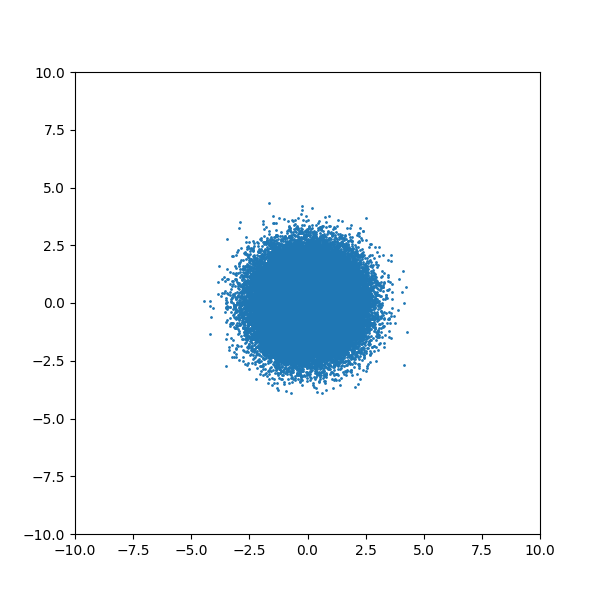
\includegraphics[width=0.19\textwidth]{result/ddpm_frame_0.png}
    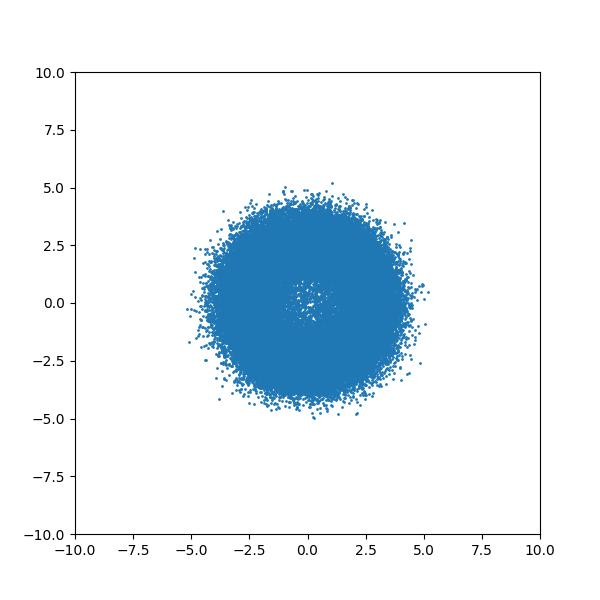
\includegraphics[width=0.19\textwidth]{result/ddpm_frame_1.png}
    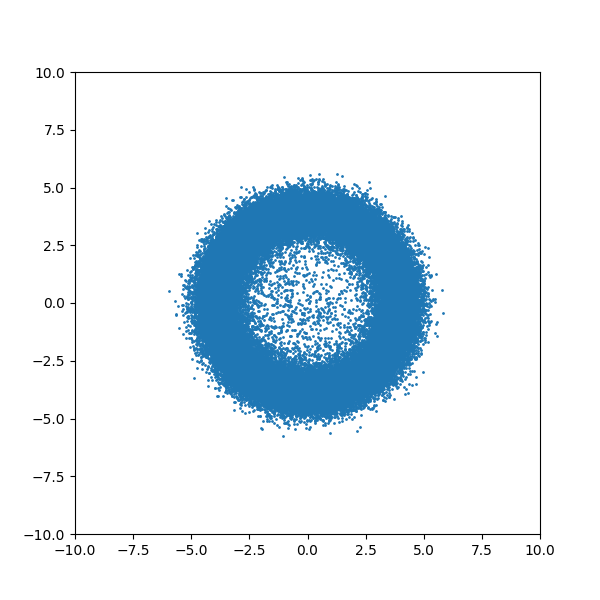
\includegraphics[width=0.19\textwidth]{result/ddpm_frame_2.png}
    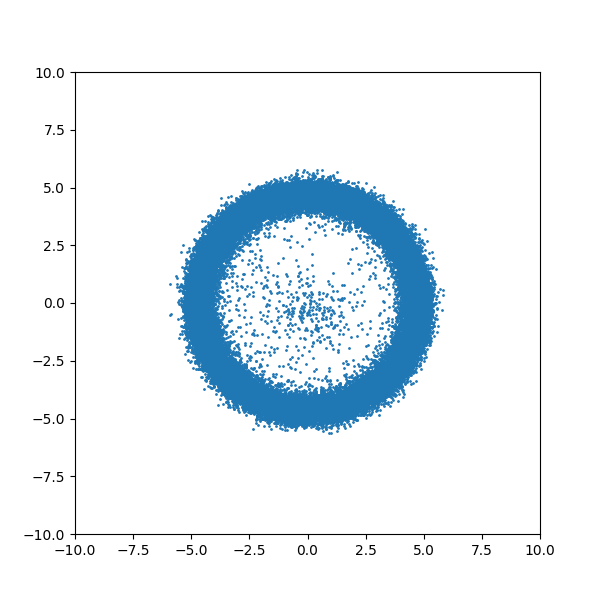
\includegraphics[width=0.19\textwidth]{result/ddpm_frame_3.png}
    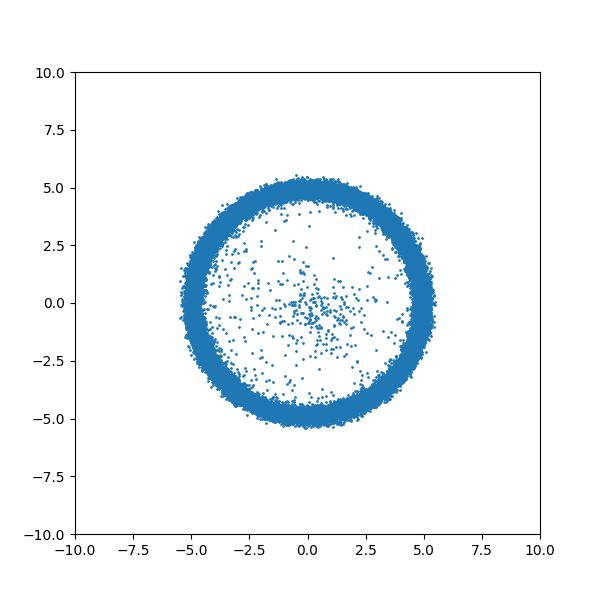
\includegraphics[width=0.19\textwidth]{result/ddpm_frame_4.png}
    \caption{DDPM reverse process snapshots (steps 99, 75, 50, 25, 0 from left to right): from Gaussian noise to the ring distribution. The full animation is saved as \texttt{result/ddpm\_ring.gif}.}
    \label{fig:ddpm_gif}
\end{figure}


% ============================================================
\section{Conditional Flow Matching}
% ============================================================

\subsection{Conditional Velocity Field}

\textbf{(a)} Given the linear interpolation path $x_t = (1-t)\,x_0 + t\,x_1$ with $x_0 \sim \mathcal{N}(0,I)$ and $x_1 \sim q_{\text{data}}$, the conditional velocity field is:
\[
    u_t(x_t \mid x_1) = \frac{dx_t}{dt} = \frac{d}{dt}\bigl[(1-t)\,x_0 + t\,x_1\bigr] = -x_0 + x_1 = x_1 - x_0.
\]

\textbf{(b)} The Conditional Flow Matching (CFM) training objective is:
\[
    \mathcal{L}_{\mathrm{CFM}}(\theta) = \mathbb{E}_{t \sim \mathcal{U}[0,1],\; x_0 \sim \mathcal{N}(0,I),\; x_1 \sim q_{\text{data}}} \left[\| v_\theta(x_t, t) - (x_1 - x_0) \|^2 \right].
\]

\textbf{Why CFM is easier to compute than the marginal flow matching loss:}
\begin{itemize}[nosep]
    \item The marginal flow matching loss requires computing the marginal velocity field $u_t(x) = \mathbb{E}[u_t(x \mid x_1) \mid X_t = x]$, which involves an intractable posterior over all possible data points $x_1$ that could have generated $x$ at time $t$.
    \item The CFM loss uses the \emph{conditional} velocity field $u_t(x_t \mid x_1) = x_1 - x_0$ directly, which is simple and closed-form for each sampled pair $(x_0, x_1)$.
    \item Lipman et al.\ (2023) proved that the gradients of the CFM loss and the marginal FM loss are identical, so minimizing CFM is equivalent to minimizing the marginal objective. This makes CFM a practical, unbiased surrogate.
\end{itemize}

\subsection{Training CFM on 8-Gaussians}

We train a velocity network (3-layer MLP with GELU activation, hidden dim 256) for 3000 iterations (batch size 4096, lr = $10^{-3}$) on the 8-Gaussians dataset (8 clusters at radius 5, std 0.2). The \texttt{cfm\_loss} and \texttt{euler\_ode\_solve} functions are implemented as described in the problem statement.

\subsection{Analysis}

\subsubsection{Effect of Euler Steps on Generation Quality}

Figure~\ref{fig:euler_steps} compares generation quality with $S \in \{1, 5, 10, 50, 100\}$ Euler steps.

\begin{figure}[H]
    \centering
    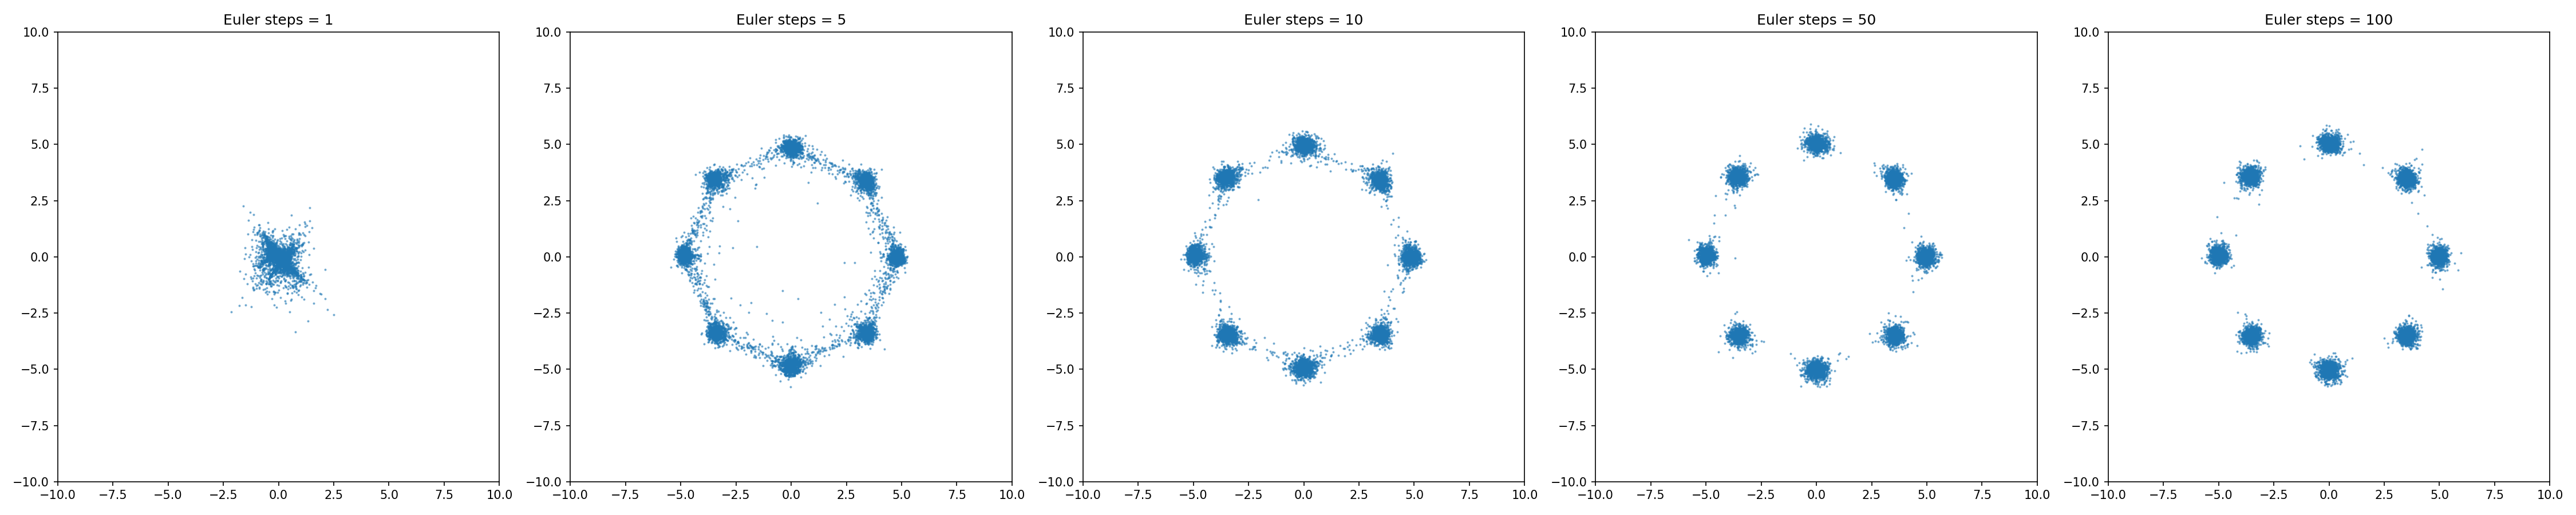
\includegraphics[width=\textwidth]{result/cfm_steps_comparison.png}
    \caption{CFM generation with different numbers of Euler integration steps.}
    \label{fig:euler_steps}
\end{figure}

\textbf{Observations:}
\begin{itemize}[nosep]
    \item \textbf{$S=1$}: Very poor quality. All samples collapse near the origin because a single linear step cannot capture the nonlinear transport from noise to data.
    \item \textbf{$S=5$}: A ring-like structure emerges, but the 8 individual clusters are not resolved. The samples are spread diffusely.
    \item \textbf{$S=10$}: The 8 modes become visible, though with noticeable spread between clusters.
    \item \textbf{$S=50$ and $S=100$}: High-quality generation with clean, well-separated 8-Gaussian clusters closely matching the ground truth.
\end{itemize}

The velocity field learned by CFM is nonlinear---it must ``steer'' particles from a broad Gaussian toward 8 concentrated targets. With too few Euler steps, the piecewise-linear approximation introduces large discretization errors, especially in regions where the velocity field changes rapidly. Beyond $S \approx 50$, the improvement is marginal.

\subsubsection{Velocity Field Visualization}

Figure~\ref{fig:velocity_field} shows the learned velocity field $v_\theta(x, t)$ at $t = 0, 0.25, 0.5, 0.75$.

\begin{figure}[H]
    \centering
    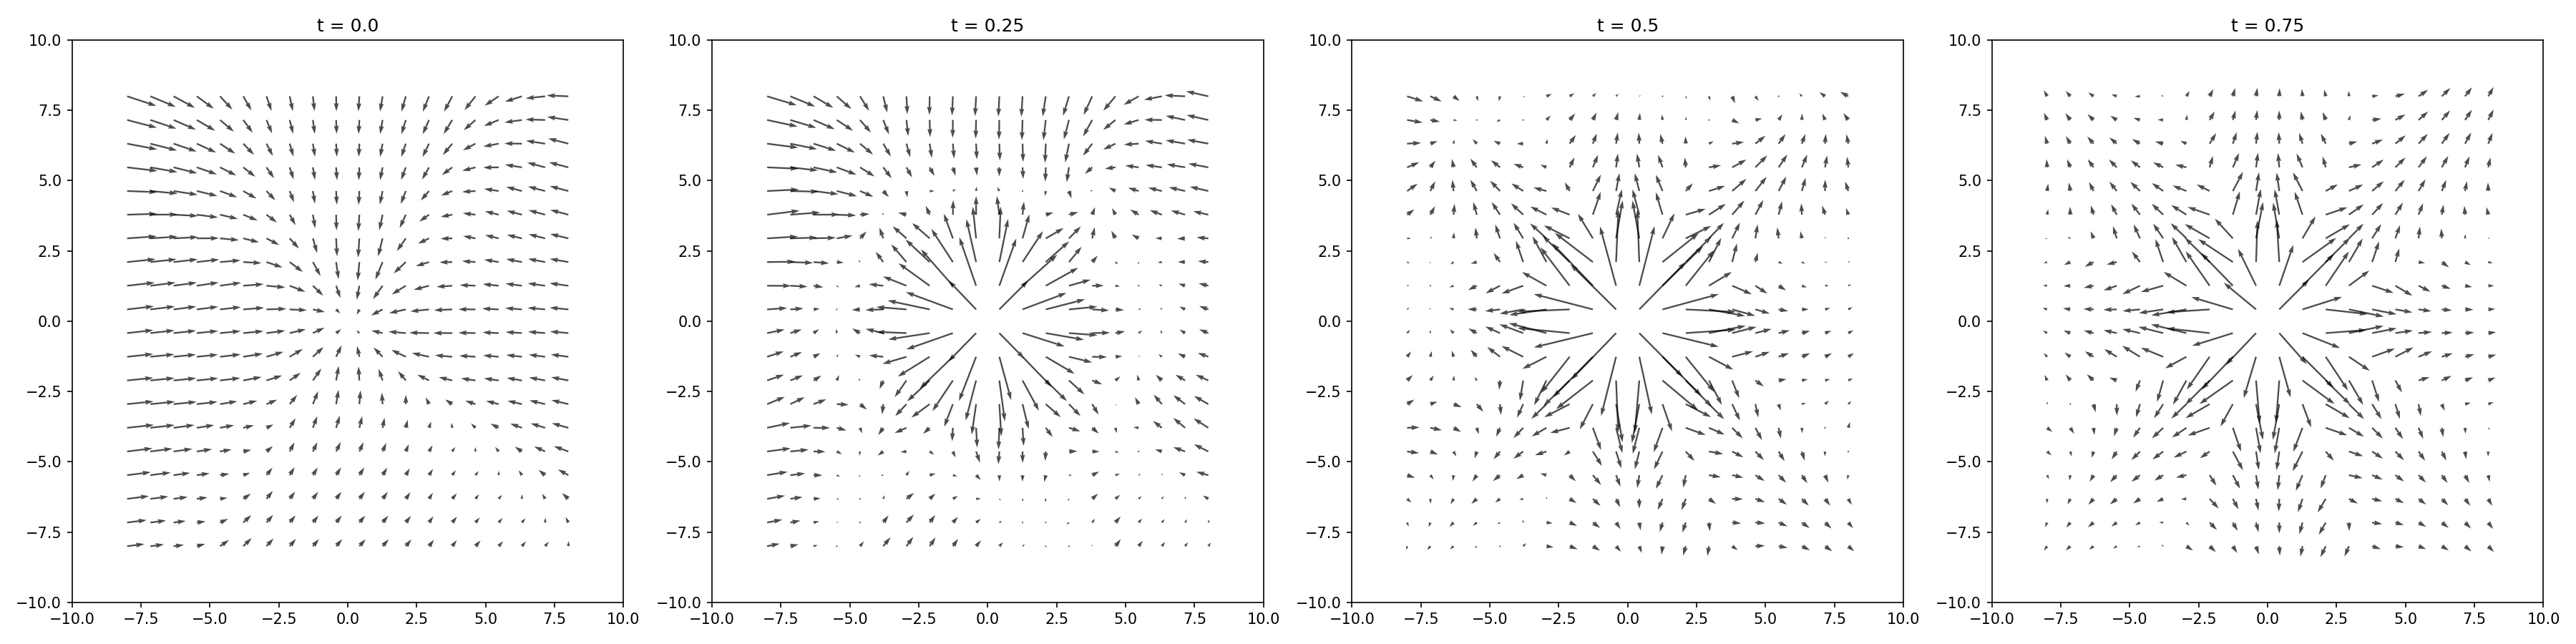
\includegraphics[width=\textwidth]{result/cfm_velocity_field.png}
    \caption{Learned velocity field at different time steps.}
    \label{fig:velocity_field}
\end{figure}

\textbf{Observations:}
\begin{itemize}[nosep]
    \item \textbf{$t=0$}: The velocity vectors are relatively uniform and point outward in all directions, broadly transporting the Gaussian noise distribution toward the periphery where the data modes lie.
    \item \textbf{$t=0.25$}: The field begins to show 8-fold structure. Velocities start converging toward the 8 cluster directions.
    \item \textbf{$t=0.5$}: The 8-mode convergence pattern is clearly visible. Vectors in between modes redirect particles toward the nearest cluster.
    \item \textbf{$t=0.75$}: The velocity field is highly localized around each mode, performing fine-grained adjustments to concentrate samples at the exact cluster centers.
\end{itemize}

In summary, the velocity field transitions from \textbf{global transport} (spreading noise outward) to \textbf{local refinement} (concentrating samples at target modes), reflecting the progressive nature of the flow.


% ============================================================
\section{Mean Flow}
% ============================================================

\subsection{MeanFlow Identity}

Define the mean velocity from time 0 to $t$ along an ODE trajectory:
\[
    \bar{u}(z_t, t) = \frac{z_t - z_0}{t}, \quad t > 0.
\]

\textbf{(a) Derivation of the MeanFlow Identity.}

From the ODE $dz_t/dt = v(z_t, t)$, we have:
\[
    z_t = z_0 + \int_0^t v(z_s, s)\, ds
    \quad \Longrightarrow \quad
    z_t - z_0 = \int_0^t v(z_s, s)\, ds.
\]
Thus:
\[
    \bar{u}(z_t, t) = \frac{z_t - z_0}{t} = \frac{1}{t}\int_0^t v(z_s, s)\, ds.
\]
We can write $z_t - z_0 = t \cdot \bar{u}(z_t, t)$. Differentiating both sides with respect to $t$ along the ODE trajectory:
\[
    \frac{d}{dt}\bigl[t \cdot \bar{u}\bigr] = \frac{d(z_t - z_0)}{dt} = v(z_t, t).
\]
Expanding the left-hand side by the product rule:
\[
    \bar{u} + t \cdot \frac{d\bar{u}}{dt} = v(z_t, t).
\]
Rearranging:
\[
    \boxed{\bar{u}(z_t, t) = v(z_t, t) - t\,\frac{d\bar{u}(z_t, t)}{dt}.}
\]

\textbf{(b) Limit as $t \to 0^+$.}

Applying L'H\^opital's rule to $\bar{u}(z_t, t) = (z_t - z_0)/t$, which is of the form $0/0$ as $t \to 0^+$:
\[
    \lim_{t \to 0^+} \frac{z_t - z_0}{t} = \lim_{t \to 0^+} \frac{dz_t/dt}{1} = \lim_{t \to 0^+} v(z_t, t) = v(z_0, 0).
\]
Hence $\lim_{t \to 0^+} \bar{u}(z_t, t) = v(z_0, 0)$: the mean velocity at the start equals the instantaneous velocity.

\textbf{(c) At $t=1$: one-step generation.}

By definition:
\[
    \bar{u}(z_1, 1) = \frac{z_1 - z_0}{1} = z_1 - z_0.
\]
If we had access to a perfect mean velocity predictor $\bar{u}(z_1, 1)$, one-step generation would be:
\[
    z_1 = z_0 + \bar{u}(z_1, 1).
\]

\textbf{Circular dependency.} However, computing $\bar{u}(z_1, 1)$ requires knowing the endpoint $z_1$, which is exactly what we are trying to generate. This creates a circular dependency: we need $z_1$ to compute the mean velocity, but we need the mean velocity to obtain $z_1$.

\textbf{Workaround.} To break this circularity, we train a \emph{displacement network} $D_\theta(z_0) \approx z_1 - z_0$ that predicts the full displacement from noise to data \emph{given only} the starting noise $z_0$. Training data consists of trajectory pairs $(z_0, z_1)$ generated by running the multi-step ODE solver. At inference time, one-step generation is simply:
\[
    z_1 = z_0 + D_\theta(z_0).
\]
This avoids the circular dependency but introduces an approximation, since $D_\theta$ must learn the inherently multi-modal mapping from noise to data. More sophisticated approaches (e.g., using the MeanFlow Identity as a self-consistency loss, as in Geng et al., 2025) can further improve quality.

\subsection{Verification and One-Step Generation}

\subsubsection{Numerical Verification of the MeanFlow Identity}

We generate ODE trajectories using 100-step Euler integration and compute three quantities along a sample trajectory: the mean velocity $\bar{u}(z_t, t)$, the instantaneous velocity $v(z_t, t)$, and the right-hand side of the identity $v(z_t, t) - t \cdot d\bar{u}/dt$.

\begin{figure}[H]
    \centering
    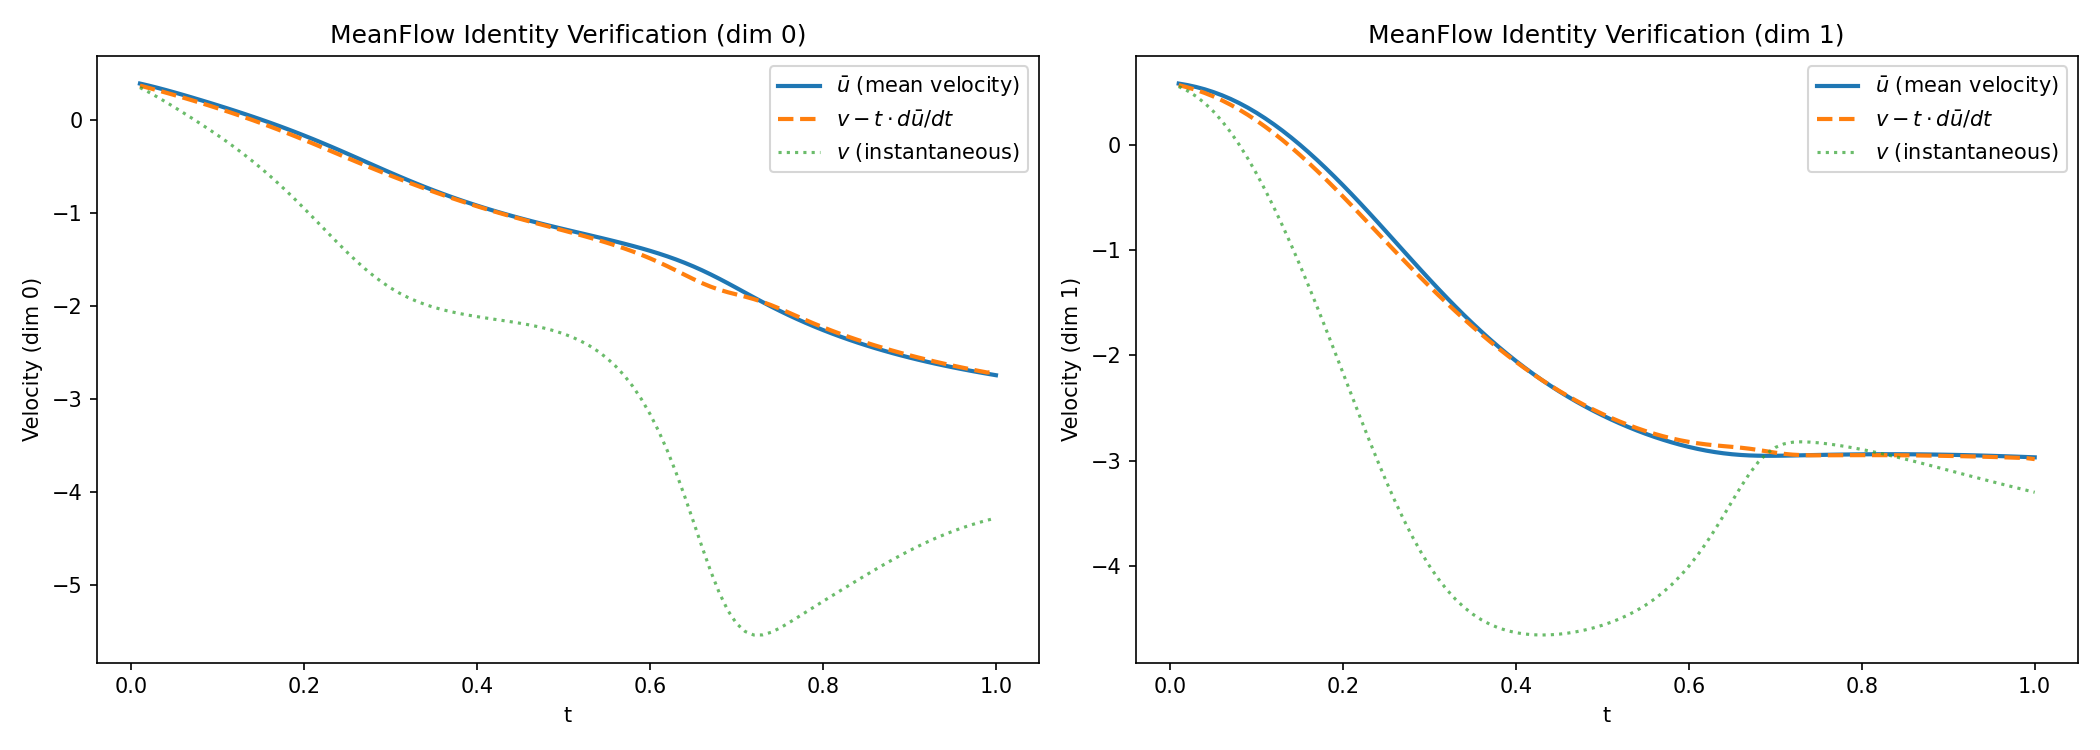
\includegraphics[width=\textwidth]{result/meanflow_identity_verification.png}
    \caption{Numerical verification of the MeanFlow Identity. The solid blue curve ($\bar{u}$) and dashed orange curve ($v - t \cdot d\bar{u}/dt$) overlap closely, confirming $\bar{u} \approx v - t \cdot d\bar{u}/dt$.}
    \label{fig:meanflow_verify}
\end{figure}

\textbf{Observation.} As shown in Figure~\ref{fig:meanflow_verify}, the mean velocity $\bar{u}$ (solid blue) and the quantity $v - t \cdot d\bar{u}/dt$ (dashed orange) are nearly identical across the entire trajectory for both dimensions. The instantaneous velocity $v$ (dotted green) differs significantly from $\bar{u}$, confirming that the mean and instantaneous velocities are distinct quantities. The close agreement between $\bar{u}$ and $v - t \cdot d\bar{u}/dt$ numerically validates the MeanFlow Identity.

\subsubsection{One-Step Generation Comparison}

We train a displacement network $D_\theta(z_0)$ (3-layer MLP, hidden dim 256) on 100,000 trajectory pairs for 50 epochs, then compare 100-step ODE generation with 1-step Mean Flow generation.

\begin{figure}[H]
    \centering
    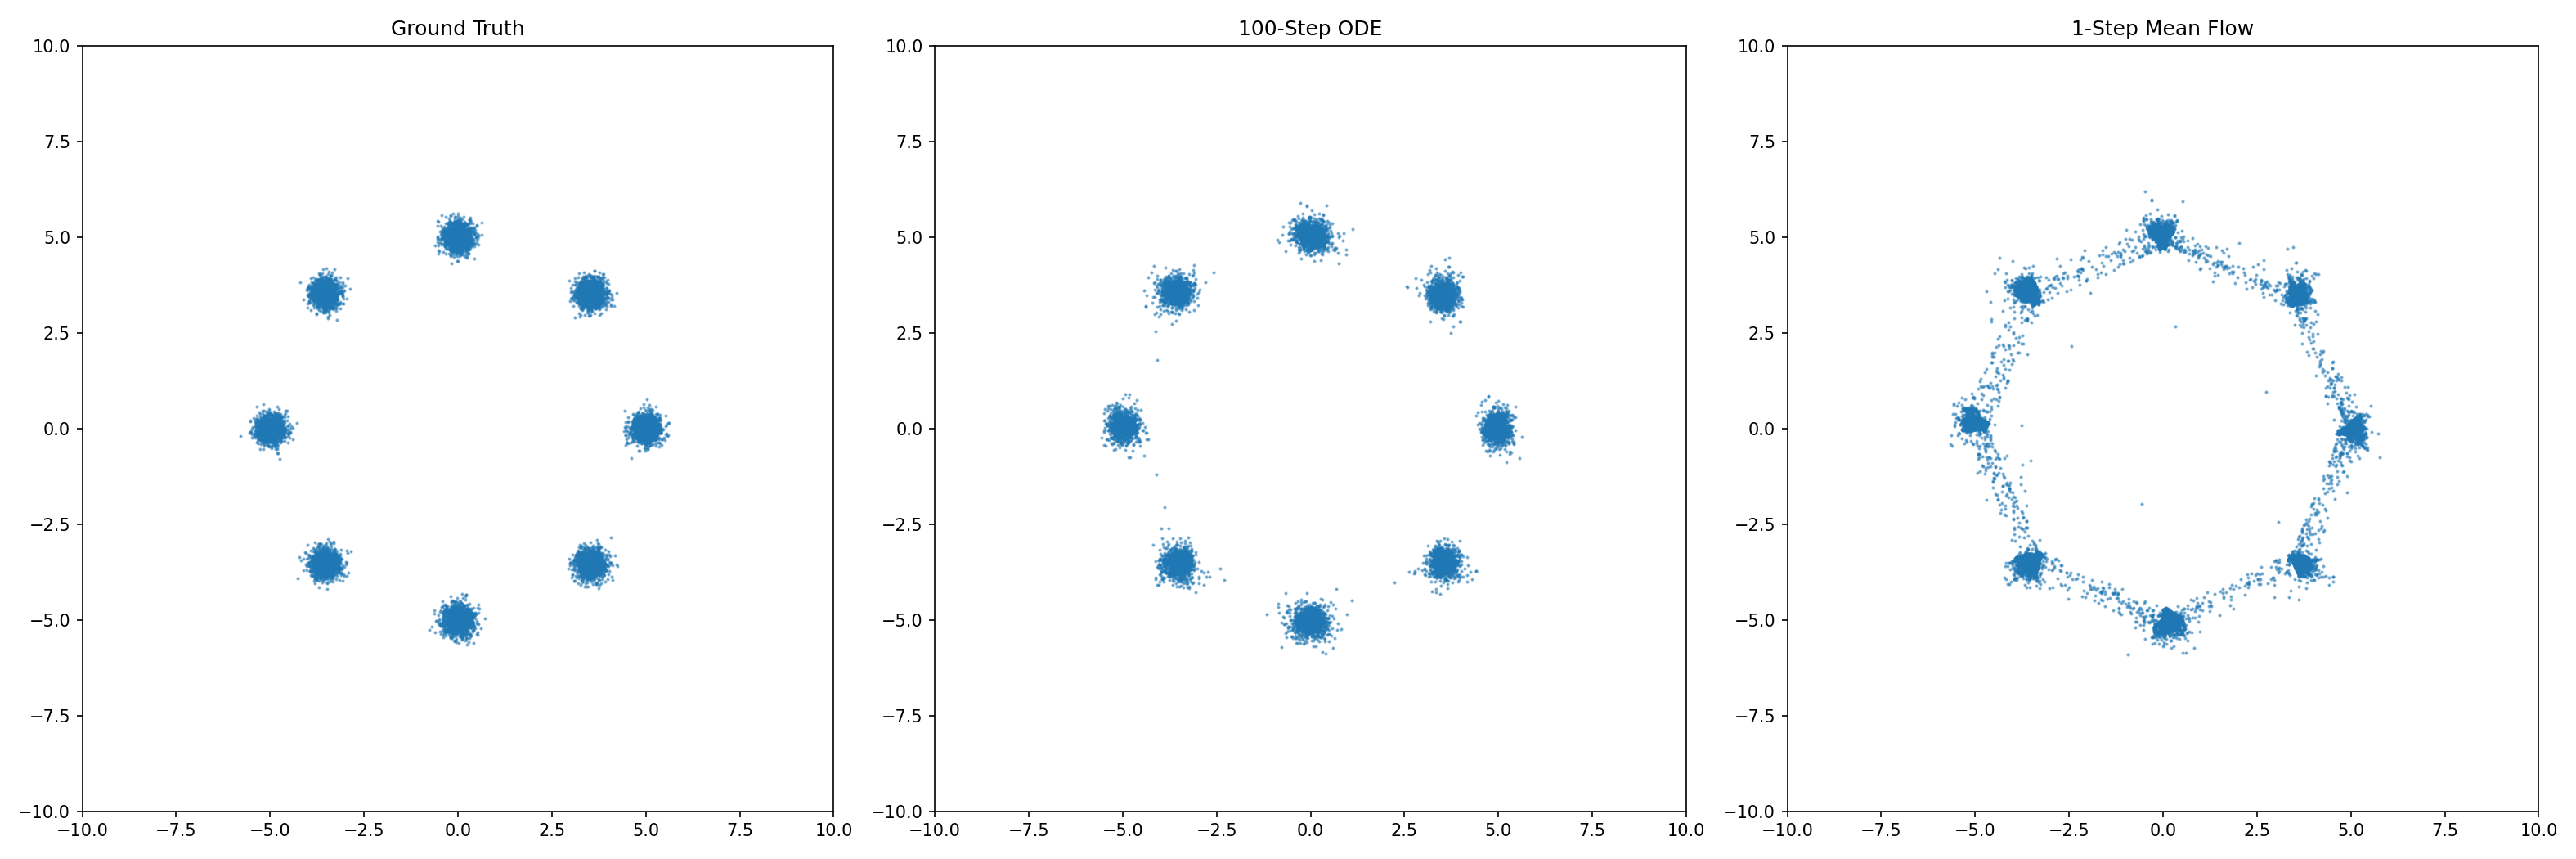
\includegraphics[width=\textwidth]{result/meanflow_one_step_comparison.png}
    \caption{Comparison of ground truth (left), 100-step ODE generation (middle), and 1-step Mean Flow generation (right).}
    \label{fig:one_step}
\end{figure}

\textbf{Observations:}
\begin{itemize}[nosep]
    \item \textbf{100-step ODE} produces clean, well-separated 8-Gaussian clusters that closely match the ground truth.
    \item \textbf{1-step Mean Flow} captures the correct locations of the 8 modes (samples are at radius $\approx 5$), but with significantly more spread. Instead of 8 discrete clusters, the samples form a ring-like distribution connecting the modes.
\end{itemize}

\textbf{Discussion.} The quality gap arises because the mapping from Gaussian noise to 8-Gaussians is inherently \emph{multi-modal}: a single noise vector $z_0$ could plausibly map to any of the 8 clusters, depending on the ODE trajectory. The displacement network $D_\theta(z_0)$ must learn this one-to-many mapping as a deterministic function, which forces it to average across modes, producing blurred inter-mode samples. The 100-step ODE avoids this issue because it makes a series of small, locally unambiguous updates.

This quality gap motivates more advanced Mean Flow training strategies (e.g., the self-consistency approach of Geng et al., 2025) that can improve one-step generation quality by leveraging the MeanFlow Identity during training rather than relying solely on distillation from pre-computed trajectories.


% ============================================================
\section*{References}
% ============================================================
\begin{itemize}[nosep]
    \item Ho J, Jain A, Abbeel P. \textit{Denoising diffusion probabilistic models}. NeurIPS, 2020.
    \item Lipman Y, Chen R T Q, Ben-Hamu H, et al. \textit{Flow matching for generative modeling}. ICLR, 2023.
    \item Geng Z, Pokle A, Luo W, et al. \textit{Mean Flows for one-step generative modeling}. arXiv:2505.13447, 2025.
\end{itemize}

\end{document}
